\documentclass{article}

\usepackage{tikz}
\usetikzlibrary{shapes,arrows}
\begin{document}

\centering
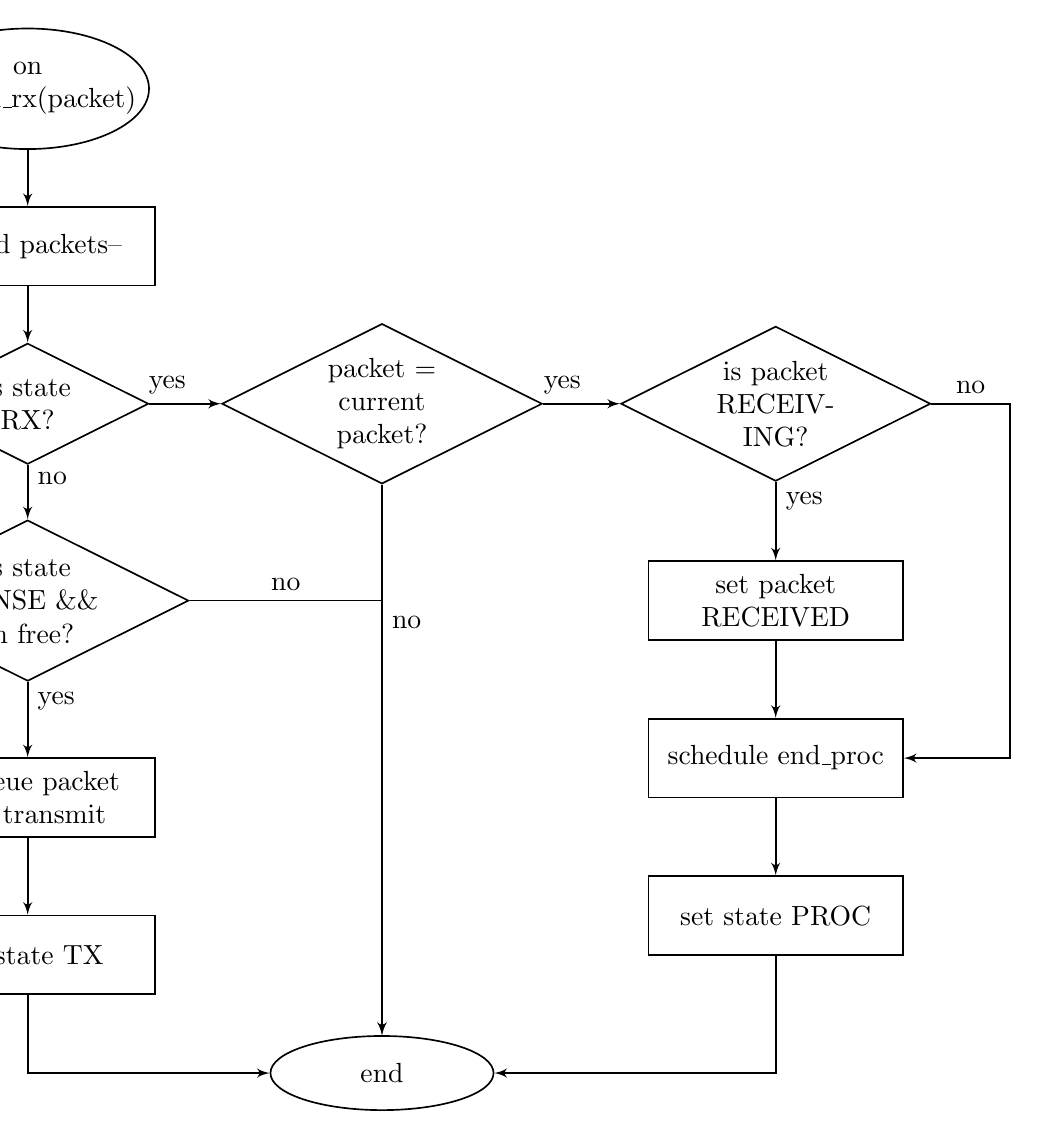
\begin{tikzpicture}[node distance = 2cm, auto, trim left, semithick]
    \tikzstyle{terminator} = [ellipse, draw,
    text width=4.5em, text centered, inner sep=6pt]
  \tikzstyle{decision} = [diamond, draw,
    text width=5em,text centered, node distance=3cm, inner sep=0pt, aspect=2]
  \tikzstyle{block} = [rectangle, draw, text width=3cm, text centered, minimum width=3cm,
    minimum height=1cm]
  \tikzstyle{line} = [draw, -latex']

  % Place nodes
  \node [terminator, text width=5em] (init) {on end\_rx(packet)};
  \node [block, below of=init, node distance=2cm] (subrcv) {sensed
    packets-- };
  \node [decision, below of=subrcv,node distance=2cm] (rx) {is state
    RX?};
  \node [decision, right of=rx, node distance=4.5cm] (iscurr)
        {packet = current packet?};

  \node [decision, right of=iscurr, node distance=5cm] (rcv) {is packet RECEIVING?};
  \node [block, below of=rcv, node distance=2.5cm] (setrcv) {set packet
    RECEIVED};
  \node [block, below of=setrcv, node distance=2cm] (sched_proc) {schedule end\_proc};
  \node [block, below of=sched_proc, node distance=2cm] (setproc) {set state PROC};
  \node [decision, below of=rx, text width=5.5em, node distance=2.5cm] (sense) {is
    state SENSE \&\& ch free?};

  \node [block, below of=sense, node distance=2.5cm] (tx) {dequeue
    packet and transmit};
  \node [block, below of=tx, node distance=2cm] (settx) {set state TX};

  \node [terminator, below of=iscurr, node distance=8.5cm] (end) {end};

  % Draw edges
  \path [line] (init) -- (subrcv);

  \path [line] (rx) -- node [near start] {yes} (iscurr);
  \path [line] (rx) -- node [near start] {no} (sense);

  \path [line] (iscurr) -- node [near start] {yes} (rcv);
  \path [line] (rcv.east) -| node [near start] {no} ++(1cm,0) |- (sched_proc);

  \path [line] (setrcv) -- (sched_proc);
  \path [line] (rcv) -- node [near start] {yes} (setrcv);
  \path [line] (iscurr) -- node [near start] {no}  (end);

  \path [line] (sched_proc) -- (setproc);
  \path [line] (setproc) |- (end);

  \path [line] (subrcv) -- (rx);

  \path [line] (sense) -- node [near start] {yes} (tx);
  \path [line] (sense) -| node [near start] {no} (end);

  \path [line] (tx) -- (settx);
  \path [line] (settx) |- (end);

\end{tikzpicture}


\end{document}
